\documentclass[preview]{standalone}

\usepackage{amsmath}
\usepackage{amssymb}
\usepackage{bettelini}
\usepackage{stellar}
\usepackage{tikz}
\usepackage{definitions}

\begin{document}

\id{settheory-definitions}
\genpage

% Russel's paradox

\section{Basic definitions}

\begin{snippetdefinition}{cardinality-definition}{Cardinality}
    The \textit{cardinality} of a set \(A\), denoted \(|A|\),
    is the amount of elements it contains.
\end{snippetdefinition}

\begin{snippetdefinition}{subset-definition}{Subset}
    If \(A\) and \(B\) are sets, then \(A\) is a \textit{subset} of \(B\)
    (\(A \origsubseteq B\)), if all the elements of \(A\) are also in \(B\).
\end{snippetdefinition}

\begin{snippetdefinition}{proper-subset-definition}{Proper Subset}
    Given two sets \(A\) and \(B\), if \(A \subseteq B\) but \(A \neq B\),
    then \(A\) is a \textit{proper} (or \textit{strict}) subset of \(B\)
    \[
        A \origsubset B
    \]
\end{snippetdefinition}

\begin{snippetdefinition}{power-set-definition}{Power set}
    If \(B\) is a set, then the \textit{power set} \(\mathcal{P}(B)\)
    is defined as the set of all subsets of \(B\)
    \[
        \mathcal{P}(B)=\{A \suchthat A\subseteq B\}
    \]
\end{snippetdefinition}

\begin{snippetdefinition}{union-definition}{Union}
    If \(A\) and \(B\) are sets, then their \textit{union} is
    \[
        A \cup B = \{x \suchthat x \in A \lor x \in B\}
    \]
\end{snippetdefinition}

\begin{snippetdefinition}{intersection-definition}{Intersection}
    If \(A\) and \(B\) are sets, then their \textit{intersection} is
    \[
        A \cap B = \{x \suchthat x \in A \land x \in B\}
    \]
\end{snippetdefinition}

\begin{snippetdefinition}{difference-definition}{Difference}
    If \(A\) and \(B\) are sets, then their \textit{difference} is
    \[
        A \backslash B = \{x \suchthat x \in A \land x \notin B\}
    \]
\end{snippetdefinition}

\begin{snippet}{set-union-intersection-difference-illustration}
    \begin{center}
        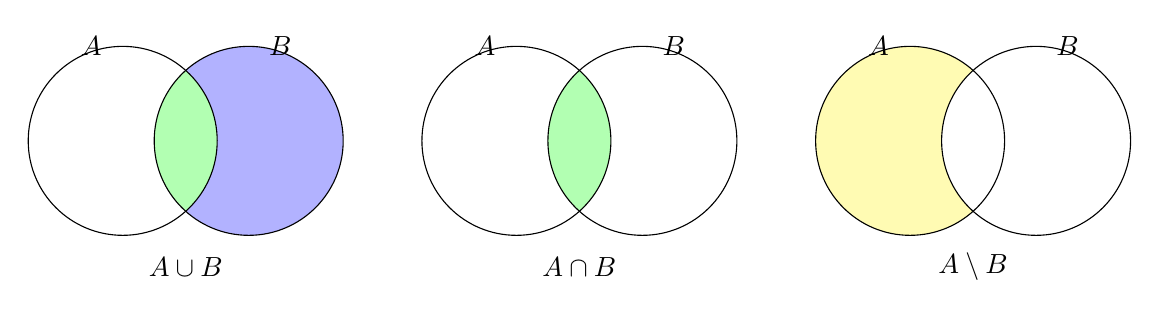
\begin{tikzpicture}
            % Union A ∪ B
            \begin{scope}[shift={(-5,0)}, scale=0.8]
                \fill[white] (-1,0) circle (1.5);
                \fill[blue!30] (1,0) circle (1.5);
                \begin{scope}
                    \clip (-1,0) circle (1.5);
                    \fill[green!30] (1,0) circle (1.5);
                \end{scope}
                \draw (-1,0) circle (1.5);
                \draw (1,0) circle (1.5);
                \node at (-1.5, 1.5) {$A$};
                \node at (1.5, 1.5) {$B$};
                \node at (0, -2) {$A \cup B$};
            \end{scope}
        
            % Intersection A ∩ B (only middle part)
            \begin{scope}[shift={(0,0)}, scale=0.8]
                \fill[white] (-1,0) circle (1.5);
                \fill[white] (1,0) circle (1.5);
                \begin{scope}
                    \clip (-1,0) circle (1.5);
                    \fill[green!30] (1,0) circle (1.5);
                \end{scope}
                \draw (-1,0) circle (1.5);
                \draw (1,0) circle (1.5);
                \node at (-1.5, 1.5) {$A$};
                \node at (1.5, 1.5) {$B$};
                \node at (0, -2) {$A \cap B$};
            \end{scope}
        
            % Difference A \ B (same as before)
            \begin{scope}[shift={(5,0)}, scale=0.8]
                \fill[yellow!30] (-1,0) circle (1.5);
                \fill[white] (1,0) circle (1.5);
                \begin{scope}
                    \clip (1,0) circle (1.5);
                    \fill[white] (-1,0) circle (1.5);
                \end{scope}
                \draw (-1,0) circle (1.5);
                \draw (1,0) circle (1.5);
                \node at (-1.5, 1.5) {$A$};
                \node at (1.5, 1.5) {$B$};
                \node at (0, -2) {$A \setminus B$};
            \end{scope}
        \end{tikzpicture}
    \end{center}
\end{snippet}

\begin{snippetdefinition}{disjoint-sets-definition}{Disjoint Sets}
    If \(A\) and \(B\) are sets and \(A \intersection B = \emptyset \), then \(A\)
    and \(B\) are \textit{disjoint sets}.
\end{snippetdefinition}

\begin{snippetdefinition}{cartesian-product-two-sets-definition}{Cartesian Product of two sets}
    [\{
        "generalizations": ["cartesian-product-definition"]
    \}]
    If \(A\) and \(B\) are sets, then their \textit{cartesian product} is
    \[
        A\times B = \{(x,y) \suchthat x \in A \land y \in B\}
    \]
    which is the set of all possible \textit{ordered pairs}.
\end{snippetdefinition}

\begin{snippetdefinition}{cartesian-product-definition}{Cartesian Product}
    Given \(n\) sets \(A_1, A_2, \ldots, A_2\),
    their \textit{cartesian product} \(A_1 \times A_2 \times \cdots \times A_n\)
    is the set of ordered \(n\)-tuples \((a_1, a_2, \ldots, a_n)\) with \(a_i\in A_i\).
\end{snippetdefinition}

\begin{snippetdefinition}{cartesian-power-definition}{Cartesian Power}
    Given a set \(A\), \(A^n=\underbrace{A \cartesianprod A \cartesianprod \cdots \cartesianprod A}_n\).
\end{snippetdefinition}

\begin{snippet}{n-dimensional-plane-cartesian-power}
    The \(n\)-dimensional plane of real numbers is a cartesian power \({\realnumbers}^n\).
\end{snippet}

\begin{snippetdefinition}{complement-definition}{Complement}
    If \(A\) is a set, its \textit{complement} is
    \[
        \bar{A} = \{x \suchthat x \notin A\}
    \]
\end{snippetdefinition}

\begin{snippetdefinition}{disjoint-union-definition}{Disjoint union}
    Given sets \(A_{i\in I}\), their disjoint union is
    \[
        \bigsqcup_{i\in I}A_i= \bigcup_{i\in I}\{(x, i) \suchthat x \in A_i\}
    \]
    which consists of prdered pairs where the second element
    is the index of the set.
\end{snippetdefinition}

\section{Basic results}

\begin{snippetcorollary}{subset-of-itself}{Every set is subset of itself}
    For every set \(A\), \(A \subseteq A\).
\end{snippetcorollary}

\begin{snippetcorollary}{empty-set-is-subset-of-any-set}{Empty set is subset of any set}
    For every set \(A\),
    \(\emptyset \subseteq A\).
\end{snippetcorollary}

\begin{snippetcorollary}{subset-of-powerset}{Subset of powerset}
    For every set \(B\), \(B\in\powerset(B)\).
\end{snippetcorollary}

\begin{snippetcorollary}{set-equivalence-with-subsets}{Set equivalence with subsets}
    Let \(A\) and \(B\) be sets.
    \[ A = B \iff A \subseteq B \land B \subseteq A \]
\end{snippetcorollary}

\begin{snippetcorollary}{subseteq-transitivity}{Subset transitivity}
    Let \(A\), \(B\) and \(C\) be sets.
    \[ A \subseteq B \land B \subseteq C \implies A \subseteq C \]
\end{snippetcorollary}

\begin{snippetproof}{subseteq-transitivity-proof}{subseteq-transitivity}{Subset transitivity}
    We have \(B \subseteq C \implies \forall b \in B, b \in C\)
    and \(A \subseteq B \implies \forall a \in A, a \in B\).
    This implies that \(\forall a \in A, a \in C\) and thus \(A \subseteq C\).
\end{snippetproof}

\begin{snippetcorollary}{proper-subsets-with-subsets}{Proper subsets with subsets}
    Let \(A\) and \(B\) be sets.
    \[ A \subset B \iff A \subseteq B \land B \notsubseteq A \]
\end{snippetcorollary}

\begin{snippetcorollary}{dual-set-difference}{}
    Note that
    \[
        A \difference B = B \difference A
        \iff A = B
    \]
\end{snippetcorollary}

\begin{snippetcorollary}{subset-in-terms-of-relationships}{Subset in terms of relationships}
    \[
        A \subseteq B
        \iff
        A \union B = B
        \iff
        A \intersection B = A
        \iff
        A \difference B = \emptyset
    \]
\end{snippetcorollary}

\begin{snippetcorollary}{set-equivalence-power-set-equivalence}{Set and power set equivalence}
    let \(A\) and \(B\) be sets.
    \[ A = B \iff \powerset(A) = \powerset(B) \]
\end{snippetcorollary}

\begin{snippetproof}{set-equivalence-power-set-equivalence-proof}{set-equivalence-power-set-equivalence}{Set and power set equivalence}
    \iffproof{
        Assume \(A=B\), then \(\powerset(A) = \powerset(B)\).
    }{
        Assume \(\powerset(A) = \powerset(B)\),
        \(A \in \powerset(A)\) and \(A \in \powerset(B)\), and thus \(A \subseteq B\).
        Likewise, we can show that \(B \subseteq A\), and by
        \snippetref[set-equivalence-with-subsets][set equivalence with subsets] we have \(A=B\).
    }
\end{snippetproof}

\begin{snippettheorem}{cardinality-of-the-power-set}{Cardinality of the power set}
    Let \(A\) be a set where \(\cardinality{A} < \infty\). The cardinality of \(\powerset(A)\) is given by
    \[
        \cardinality{\powerset(A)} = 2^{\cardinality{A}}
    \]
\end{snippettheorem}

\begin{snippetproof}{cardinality-of-the-power-set-proof}{cardinality-of-the-power-set}{Cardinality of the power set}
    Let \(A\) be a set where \(\cardinality{A} < \infty\).
    TODO
\end{snippetproof}

\begin{snippetcorollary}{infinite-set-power-set-is-infinite}{Power set of infinite set is infinite}
    Let \(A\) be a set where \(\cardinality{A} = \infty\).
    \[ \cardinality{\powerset(A)} =\infty \]
\end{snippetcorollary}

\begin{snippetproof}{infinite-set-power-set-is-infinite-proof}{infinite-set-power-set-is-infinite}{Power set of infinite set is infinite}
    Let \(A\) be a set where \(\cardinality{A} = \infty\).
    Let's assume that \(\cardinality{\powerset(A)} < \infty\), then there would be a finite number of subsets of \(A\).
    This implies that there is only a maximum numbers of distinct subsets that can be formed from \(A\),
    but an infinite set should always be able to create an infinite amount of distinct subsets \lightning.
\end{snippetproof}

%Dimostrare che se A ⊆ B, B ⊆ C e almeno una delle due inclusioni è
%stretta, allora A ⊂ C.

\end{document}
